%!TEX root = ../nips_2017.tex





\section{Preliminaries}

%%%%%%%%%%%%%%%%%%%%%%%%%%%%%%%%%%%%%%%%%%%%%%%%%%%%%%%%%%%%%%%%%%%%%%%%%%%%%%%
% \paragraph{Notation:}
% \label{sub:notation}
%%%%%%%%%%%%%%%%%%%%%%%%%%%%%%%%%%%%%%%%%%%%%%%%%%%%%%%%%%%%%%%%%%%%%%%%%%%%%%%

\textbf{Notation:} For a vector $v \in \bbR^n$ we denote the $\ell_p$ norm by $\|v\|_p = \left(\sum_i |v_i|^p \right)^{1/p}$. The convolution of two vectors $v_1 \in \bbR^N$ and $v_2 \in \bbR^M$ is denoted by $v_1 \ast v_2 \in \bbR^{N + M - 1}$. We denote by $x$ the observed signals, $d$ the temporal atoms, and $z$ the sparse vector of \emph{activations}. The symbols ${\cal U}$, ${\cal E}$, ${\cal N}$, ${\cal S}$ denote the univariate uniform, exponential, Gaussian, and $\alpha$-stable distributions, respectively.

% \paragraph{Convolutional sparse coding:}
% \label{sub:csc}
\textbf{Convolutional sparse coding:} 
The CSC problem formulation adopted in this work follows the Shift Invariant Sparse Coding (SISC) model from~\cite{Grosse-etal:2007}. It is defined as follows:
%
\begin{align}
 \min_{d, z} \sum_{n=1}^{N} \Big( \frac{1}{2}\|x_{n} - \sum_{k=1}^{K}d^{k} * z_{n}^{k}\|_{2}^{2} + \lambda \sum_{k=1}^K \|z_{n}^{k}\|_1 \Big), \hspace{9pt}
 \text{s.t. } \>\> \|d^{k}\|_2^2 \leq 1 \text{  and } z_n^k \geq 0, \forall n, k
\label{eq:problem_definition} \enspace ,
\end{align}
%
where $x_{n} \in \bbR^{T}$ denotes one of the $N$ observed segments of signals, also referred to as a \emph{trials} in this paper. We denote by $T$ as the length of a trial, and $K$ the number of atoms. The aim in this model is to approximate the signals $x_n$ by the convolution of certain \emph{atoms} and their respective \emph{activations}, which are sparse. Here, $d^{k} \in \bbR^{L}$ denotes the $k$th atom of the \emph{dictionary} $d \equiv \{d^k\}_{k}$, and $z_{n}^{k} \in \bbR_+^{T-L+1}$ denotes the activation of the $k$th atom in the $n$th trial. We denote by $z \equiv \{z_n^k\}_{n,k}$.
%the collection of all the activations.

The objective function \eqref{eq:problem_definition} has two terms, an $\ell_2$ data fitting term that corresponds to assuming an additive Gaussian noise model, and a regularization term that promotes sparsity with an $\ell_1$ norm.
The regularization parameter is called $\lambda > 0$. Two constraints are also imposed. First, we ensure that $d^{k}$ lies within the unit sphere, which prevents the scale ambiguity between $d$ and $z$. Second, a positivity constraint on $z$ is imposed to be able to obtain physically meaningful activations and to avoid sign ambiguities between $d$ and $z$. This positivity constraint is not present in the original SISC model~\citep{Grosse-etal:2007}.

\begin{figure}[t]
    \centering
    \subfigure[]{
    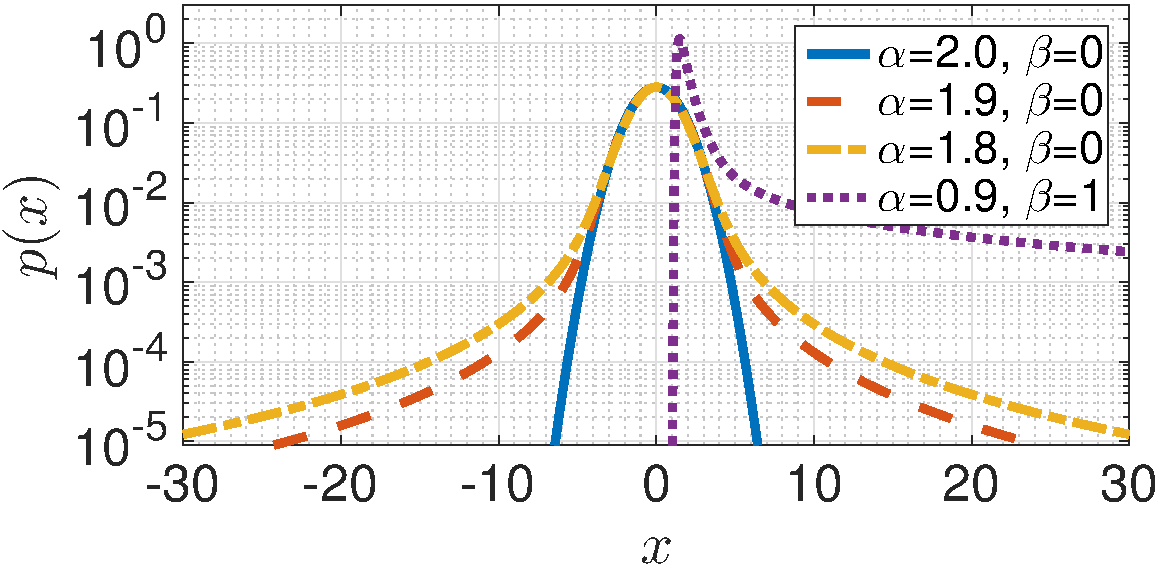
\includegraphics[width=0.31\linewidth]{figures/stablepdf3.pdf}
    \label{fig:stable_pdf}
    } \hfill
    \subfigure[]{
    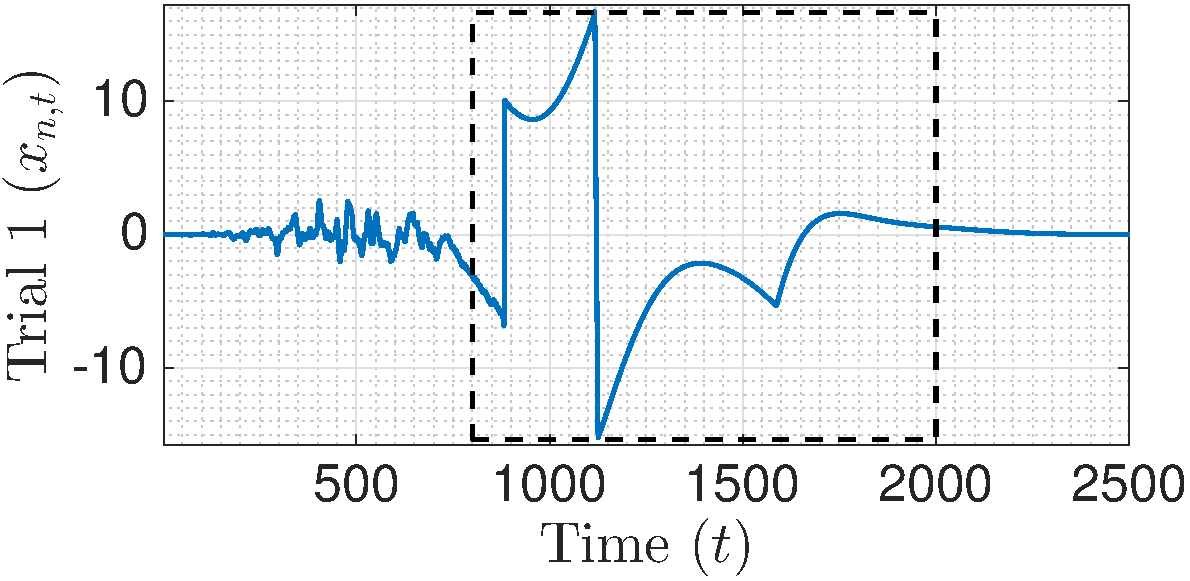
\includegraphics[width=0.31\linewidth]{figures/cfc_data1_2.pdf}
    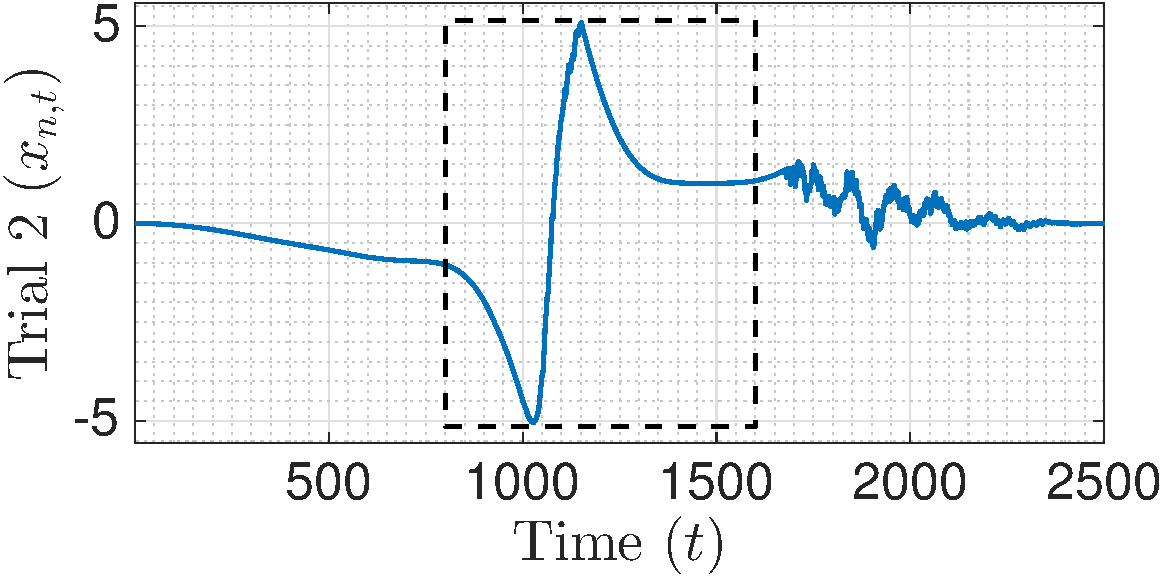
\includegraphics[width=0.31\linewidth]{figures/cfc_data2_2.pdf}
    % \includegraphics[width=0.235\linewidth]{figures/lfpdata3.pdf}
    \label{fig:artifacts}
    }
    \caption[PDSFs of $\alpha$-stable distributions and trials containing artifacts.]{(a) PDFs of $\alpha$-stable distributions. (b) Illustration of two trials from the striatal LFP data, which contain severe artifacts. The artifacts are illustrated with dashed rectangles.}
    \label{fig:pdf_lfp}
\end{figure}


% \paragraph{$\alpha$-Stable distributions:}
% \label{sub:stabledist}

% \begin{wrapfigure}{O}{0.5\columnwidth}
% %\vskip 0.2in
% \begin{center}
% % \centerline{
% % \subfigure[]{
% \vspace{-10pt}
% \includegraphics[width=0.49\columnwidth]{./figures/stablepdf.pdf}
% % }
% \end{center}
% \vspace{-15pt}
% \caption{PDFs of stable distributions.}
% \label{fig:stable_pdf} 
% \end{wrapfigure}


\textbf{$\alpha$-Stable distributions:} 
The $\alpha$-stable distributions have become increasingly popular in modeling signals that might incur large variations \citep{kuruoglu1999signal, mandelbrot2013fractals,simsekli2015alpha,wang2016delving,leglaive:hal-01416366} and have a particular importance in statistics since they appear as the limiting distributions in the generalized central limit theorem \citep{samorodnitsky1994stable}. They are characterized by four parameters: $\alpha$, $\beta$, $\sigma$, and $\mu$:
%
(i) $\alpha \in (0,2]$ is the \emph{characteristic exponent} and determines the tail thickness of the distribution: the distribution will be heavier-tailed as $\alpha$ gets smaller. 
(ii) $\beta \in [-1 ,1]$ is the \emph{skewness} parameter.
%and determines whether the distribution is right- or left-skewed
If $\beta = 0$, the distribution is symmetric.
(iii) $\sigma \in (0,\infty)$ is the \emph{scale} parameter and measures the spread of the random variable around its mode (similar to the standard deviation of a Gaussian distribution). Finally, (iv) $\mu \in (-\infty, \infty)$ is the location parameter (for $\alpha > 1$, it is simply the mean). 

The probability density function of an $\alpha$-stable distribution cannot be written in closed-form except for certain special cases; however, the characteristic function  can be written as follows:
%\begin{align*}
%x \sim {\cal S}(\alpha,\beta,\sigma,\mu) \iff \mathds{E}[\exp( i \omega x)]  = \exp(-|\sigma \omega|^\alpha \left[1+ i \sign(\omega)\beta \psi_\alpha(\omega)  \right] + i \mu \omega ) \enspace ,
%\end{align*}
where $\psi_\alpha(\omega) = \log |\omega| $ for $\alpha =1$, $\psi_\alpha(\omega) = \tan(\pi \alpha/2)$ for $\alpha \neq 1$, and $i = \sqrt{-1}$. 
%
As an important special case of the $\alpha$-stable distributions, we obtain the Gaussian distribution when $\alpha = 2$ and $\beta =0$, \textit{i.e.}\ ${\cal S}(2,0,\sigma,\mu) = {\cal N}(\mu,2 \sigma^2)$. 
%
In Fig.~\ref{fig:stable_pdf}, we illustrate the (approximately computed) \acp{PDF} of the $\alpha$-stable distribution for different values of $\alpha$ and $\beta$. The distribution becomes heavier-tailed as we decrease $\alpha$, whereas the tails vanish quickly when $\alpha=2$. 


The moments of the $\alpha$-stable distributions can only be defined up to the order $\alpha$, i.e. $\mathds{E}[|x|^p] < \infty $ if and only if $p <\alpha$, which implies the distribution has infinite variance when $\alpha<2$. Furthermore, despite the fact that the \acp{PDF} of $\alpha$-stable distributions do not admit an analytical form, it is straightforward to draw random samples from them~\citep{chambers1976method}.





\section{Alpha-Stable Convolutional Sparse Coding}

\subsection{The Model}


From a probabilistic perspective, the \ac{CSC} problem can be also formulated as a \ac{MAP} estimation problem on the following probabilistic generative model:
%
\begin{align}
z_{n,t}^k \sim {\cal E}(\lambda),
\quad x_{n,t} | z, d \sim {\cal N}( \hat{x}_{n,t},1 ),
\quad \text{ where,}
\quad \hat{x}_n \triangleq \sum_{k=1}^{K}d^{k} * z_{n}^{k} \enspace .
\label{eqn:csc_prob}
\end{align}
%
Here, $z_{n,t}^k$ denotes the $t$th element of $z_{n}^k$. We use the same notations for $x_{n,t}$ and $\hat{x}_{n,t}$. It is easy to verify that the MAP estimate for this probabilistic model, \textit{i.e.}\ $\max_{d,z} \log p(d,z|x)$, is identical to the original optimization problem defined in~\eqref{eq:problem_definition}\footnote{Note that the positivity constraint on the activations is equivalent to an exponential prior for the regularization term rather than the more common Laplacian prior.}.

It has been long known that, due to their light-tailed nature, Gaussian models often fail at handling noisy high amplitude observations or outliers~\citep{Huber81a}. As a result, the `vanilla' \ac{CSC} model turns out to be highly sensitive to outliers and impulsive noise that frequently occur in electrophysiological recordings, as illustrated in Fig.~\ref{fig:artifacts}. Possible origins of such artifacts are movement, muscle contractions, ocular blinks or electrode contact losses.
 % \umut{Mention the figure from the LFP data.} % albeit it has been shown to be successful for audio processing and computer vision applications.


% In order to be able to handle such challenging data, probabilistic models that are based on non-Gaussian heavy-tailed distributions have become increasingly popular in various domains \umut{should go to intro}. 

% \cite{samoradnitsky1994stable}

In this study, we aim at developing a probabilistic \ac{CSC} model that would be capable of modeling challenging electrophysiological signals. We propose an extension of the original CSC model defined in~\eqref{eqn:csc_prob} by replacing the light-tailed Gaussian likelihood (corresponding to the $\ell_2$ reconstruction loss in~\eqref{eq:problem_definition}) with heavy-tailed $\alpha$-stable distributions. We define the proposed probabilistic model ($\alpha$CSC) as follows:
\begin{align}
z_{n,t}^k \sim {\cal E}( \lambda),  \quad
x_{n,t} | z, d \sim {\cal S} (\alpha, 0, 1/\sqrt{2}, \hat{x}_{n,t} ) \enspace , \label{eqn:acsc_org}
\end{align}
where ${\cal S}$ denotes the $\alpha$-stable distribution.
%
%\footnote{\mainak{We remark here that even though mixture models could also be used to achive robustness, this would most likely be a worse choice compared to alpha stable distributions~\citep{swami2000non}.} \umut{I really don't think these explanations are necessary.}}. 
%
While still being able to capture the temporal structure of the observed signals via convolution, the proposed model has a richer structure and would allow large variations and outliers, thanks to the heavy-tailed $\alpha$-stable distributions. Note that the vanilla \ac{CSC} defined in \eqref{eqn:csc_prob} appears as a special case of $\alpha$CSC, as the $\alpha$-stable distribution coincides with the Gaussian distribution when $\alpha=2$. 


% \mainak{We remark here that even though mixture models could also be used to achive robustness, this would most likely be a worse choice compared to alpha stable distributions~\citep{swami2000non}. Further, even though biconvex problems have theoretical guarantees\citep{agarwal2014learning, gorski2007biconvex}, we observe that in practice, the sampling route does not come with any additional disadvantage due to our multiple restart strategy.} 



%\umut{More explanation on the model, what happens when $\alpha=2$ etc.}




% It is easy to verify that this model coincides with the Gaussian model defined above, when $\alpha=2$. 

\subsection{Maximum A-Posteriori Inference}
%  of the latent variables $d$ and $z$
Given the observed signals $x$, we are interested in the MAP estimates, defined as follows:
\begin{align}
(d^\star,z^\star) = \argmax_{d,z}  \sum_{n,t} \Bigl( \log p(x_{n,t}|d,z) + \sum_k \log p(z_{n,t}^k)  \Bigr).
\end{align}
As opposed to the Gaussian case, unfortunately, this optimization problem is not amenable to classical optimization tools, since the \ac{PDF} of the $\alpha$-stable distributions does not admit an analytical expression.  
%
As a remedy, we use the product property of the symmetric $\alpha$-stable densities \citep{samorodnitsky1994stable,godsill1999bayesian} and re-express the $\alpha$CSC model as conditionally Gaussian. It leads to:
\begin{align}
% z_{i}^k[t] &\sim {\cal E}( \lambda) \\
z_{n,t}^k \sim {\cal E}( \lambda),  \quad 
\phi_{n,t} \sim {\cal S}\Bigl(\frac{\alpha}{2},1, 2 (\cos \frac{\pi \alpha}{4})^{2/\alpha} ,0 \Bigr), \quad
x_{n,t} | z, d, \phi \sim {\cal N}\Bigl(\hat{x}_{n,t},\frac{1}{2}\phi_{n,t} \Bigr) \enspace ,
\label{eqn:sas_condgauss}
\end{align}
where $\phi$ is called the \emph{impulse} variable that is drawn from a \emph{positive} $\alpha$-stable distribution (i.e.\ $\beta =1$), whose \ac{PDF} is illustrated in Fig.~\ref{fig:stable_pdf}. It can be shown that both formulations of the $\alpha$CSC model are identical by marginalizing the joint distribution $p(x,d,z,\phi)$ over $\phi$ \cite[Proposition 1.3.1]{samorodnitsky1994stable}. 

The impulsive structure of the $\alpha$CSC model becomes more prominent in this formulation: the variances of the Gaussian observations are modulated by stable random variables with infinite variance, where the impulsiveness depends on the value of $\alpha$. 
%
It is also worth noting that when $\alpha = 2$, $\phi_{n,t}$ becomes deterministic and we can again verify that $\alpha$CSC coincides with the vanilla \ac{CSC}. 

% One of the main advantages of the augmented model \eqref{eqn:sas_condgauss} is its conditional Gaussianity

The conditionally Gaussian structure of the augmented model has a crucial practical implication: if the impulse variable $\phi$ were to be known, then the \ac{MAP} estimation problem over $d$ and $z$ in this model would turn into a `weighted' \ac{CSC} problem, which is a much easier task compared to the original problem. In order to be able to exploit this property, we propose an \ac{EM} algorithm, which iteratively maximizes a lower bound of the log-posterior $\log p(d,z|x)$, and algorithmically boils down to computing the following steps in an iterative manner:
\begin{align}
&\text{E-Step:} \hspace{20pt} {\cal B}^{(i)}(d,z) = \mathds{E}\left[\log p(x,\phi,z|d)\right]_{p(\phi|x,z^{(i)},d^{(i)})}, \\
&\text{M-Step:} \hspace{20pt} (d^{(i+1)}, z^{(i+1)}) = \argmax\nolimits_{d,z} {\cal B}^{(i)}(d,z). \label{eq:mstep}
\end{align}
where $\mathds{E}[f(x)]_{q(x)}$ denotes the expectation of a function $f$ under the distribution $q$, $i$ denotes the iterations, and ${\cal B}^{(i)}$ is a lower bound to $\log p(d,z|x)$ and it is tight at the current iterates $z^{(i)}$, $d^{(i)}$.



%

%
% Accordingly, the M-Step simplifies as well and becomes:
% %
% \begin{align}
% \min_{d,z\geq 0} \Bigl( \sum_i \sum_t \tau_i[t](x_i[t] -\hat{x}_i[t] )^2 + \lambda \sum_{k}{z_{i}^{k}}    \Bigr).
% \label{eq:mstep}
% \end{align}
% %
% We can observe that the M-step is a slight modification of our initial optimization problem~\eqref{eq:problem_definition}. We now detail computations of both E and M-steps.

% \paragraph{The E-Step:}
\textbf{The E-Step:} 
In the first step of our algorithm, we need to compute the \ac{EM} lower bound ${\cal B}$ that has the following form:
\begin{align}
{\cal B}^{(i)}(d,z) =^+ - \sum_{n=1}^N \Big( \|\sqrt{w_{n}^{(i)}} \odot (x_{n} - \sum_{k=1}^{K}d^{k} * z_{n}^{k})\|_{2}^{2} + \lambda \sum_{k=1}^K{\|z_{n}^{k}\|_1}\Big),
\end{align}
where $=^+$ denotes equality up to additive constants, $\odot$ denotes the Hadamard (element-wise) product, and the square-root operator is also defined element-wise. Here, $w_{n}^{(i)} \in \bbR^T_+$ are the \emph{weights} that are defined as follows: $w_{n,t}^{(i)} \triangleq \mathds{E}\left[1/{\phi_{n,t}}\right]_{p(\phi|x,z^{(i)},d^{(i)})}$. As the variables $\phi_{n,t}$ are expected to be large when $\hat{x}_{n,t}$ cannot explain the observation $x_{n,t}$ -- typically due to a corruption or a high noise -- the weights will accordingly suppress the importance of the particular point $x_{n,t}$. Therefore, the overall approach will be more robust to corrupted data than the Gaussian models where all weights would be deterministic and equal to $0.5$. 

% \utodo{more semantics about this weight.} 

 
%
% \begin{align}
%  \tau_i[t]^{(i)} \triangleq \mathds{E}\left[\frac1{\phi_i[t]}\right]_{p(\phi|x,z^{(i)},d^{(i)})}. \label{eqn:tau_exp}
% \end{align} 

% {% tex broke the page here!!!!
% \parfillskip=0pt
% \parskip=0pt
% \par}

    \begin{algorithm}[H]
      \begin{algorithmic}[1] %(regularization parameter), (number of EM iterations), (number of MCMC iterations)
      \REQUIRE Regularization: $\lambda \in \real_+$, Num. atoms: $K$, Atom length: $L$, Num. iterations: $I$ , $J$, $M$
        %\STATE $\hat{d \in \real^{K \times L}} \leftarrow 0$, $\hat{z} \in \real^{K \times N \times T} \leftarrow 0$
        \FOR{$i=1$ to $I$}
          \STATE \textit{\color{blue} /* E-step: */} %Estimate $w^{(i)}$ as follows:
          \FOR{$j=1$ to $J$}
          \STATE Draw $\phi_{n,t}^{(i,j)}$ via MCMC \eqref{eqn:mcmc_acc}
          \ENDFOR
          \STATE $w_{n,t}^{(i)} \approx (1/J) \sum\nolimits_{j=1}^{J} 1/{\phi_{n,t}^{(i,j)}}$
          % \ENDFOR
          \STATE \textit{\color{blue} /* M-step: */} %Estimate $d^{(i)}, z^{(i)}$ as follows:
              \FOR{$m=1$ to $M$}
                  \STATE $z^{(i)}$ = L-BFGS-B on \eqref{eq:problem_definition_z}
                  \STATE $d^{(i)}$ = L-BFGS-B on the dual of \eqref{eq:problem_definition_d}
              \ENDFOR
        \ENDFOR
        \RETURN $w^{(I)}$, $d^{(I)}$, $z^{(I)}$
        \end{algorithmic}
        \caption{$\alpha$-stable Convolutional Sparse Coding}
        \label{alg:alpha_csc}
    \end{algorithm}

Unfortunately, the weights $w^{(i)}$ cannot be computed analytically, therefore we need to resort to
approximate methods. In this study, we develop a \ac{MCMC} method to approximately compute the weights, where we approximate the intractable expectations with a finite sample average, given as follows: $w_{n,t}^{(i)} \approx (1/{J}) \sum_{j=1}^{J} 1/{\phi_{n,t}^{(i,j)}}$, where $\phi_{n,t}^{(i,j)}$ are some samples that are ideally drawn from the posterior distribution $p(\phi|x,z^{(i)},d^{(i)})$. Unfortunately, directly drawing samples from the posterior distribution of $\phi$ is not tractable either, and therefore, we develop a \emph{Metropolis-Hastings} algorithm \citep{chib1995understanding}, that asymptotically generates samples from the \emph{target} distribution $p(\phi|\cdot)$ in two steps. In the $j$-th iteration of this algorithm, we first draw a random sample for each $n$ and $t$ from the prior distribution (cf.\ \eqref{eqn:sas_condgauss}), \textit{i.e.}, $\phi_{n,t}'\sim p(\phi_{n,t})$. We then compute an acceptance probability for each $\phi_{n,t}'$ that is defined as follows:
%
\begin{align}
  % \text{acc}(\phi_{n,t}^{(i,j)} \rightarrow \phi_{n,t}' ) \triangleq \exp \Bigl\{ (\log \phi_{n,t}^{(i,j)} - \log \phi_{n,t}')/2 + (x_{n,t} - \hat{x}^{(i)}_{n,t})^2 (1/{\phi_{n,t}^{(i,j)}} - 1/{\phi_{n,t}'}) \Bigr\}
  \text{acc}(\phi_{n,t}^{(i,j)} \rightarrow \phi_{n,t}' ) \triangleq \min \Bigl\{1, {p(x_{n,t}|d^{(i)},z^{(i)},\phi'_{n,t})}/{p(x_{n,t}|d^{(i)},z^{(i)},\phi_{n,t}^{(i,j)})} \Bigr\} \label{eqn:mcmc_acc}
\end{align}
%
where $j$ denotes the iteration number of the \ac{MCMC} algorithm. 
% and $\hat{x}^{(i)}_{n}$ is computed as in \eqref{eqn:csc_prob} by using the current iterates $d^{(i)}$ and $z^{(i)}$. 
Finally, we draw a uniform random number $u_{n,t} \sim {\cal U}([0, 1])$ for each $n$ and $t$. If $u_{n,t} < \text{acc}(\phi_{n,t}^{(i)} \rightarrow \phi_{n,t}')$, we accept the sample and set $\phi_{n,t}^{(i+1)} = \phi_{n,t}'$; otherwise we reject the sample and set $\phi_{n,t}^{(i+1)} = \phi_{n,t}^{(i)}$. This procedure forms a Markov chain that leaves the target distribution $p(\phi|\cdot)$ invariant, where under mild ergodicity conditions, it can be shown that the finite-sample averages converge to their true values when $J$ goes to infinity \citep{Liu2008}. More detailed explanation of this procedure is given in Section~\ref{sec:e-step}.

%

%
% \ag{maths / derivations in appendix? it's too fast for me.}
% To simplify notation, from now on, we will use $\tau_{i} \in \bbR^{T}$ to denote all the activations for one sample.